\makeatletter
\def\input@path{{../../}}
\makeatother
\documentclass[../../main.tex]{subfiles}

\graphicspath{
	{../../img/}
	{../img/}
	{img/}
}

\begin{document}
\subsection{Связь ПовИ-2 с ПовИ-1}

Рассмотрим ПовИ-2 вида \[\iint\limits_\pi R(x, y, z)dxdy.\]

На выбранной стороне поверхности $\pi$ проводится разбиение на части $\pi_k,\
 k=\overline{1,n},$ при этом $\Delta s_k =\text{пл. }\pi_k.$
От произвольной точки $M_k(x_k, y_k, z_k)\in\pi_k$ поверхность $\pi_k$ 
проецируется на плоскость $Oxy,$ то есть $D_k = \text{пр}_{Oxy} \pi_k,$ где
 $\Delta\sigma_k = \text{пл. }D_k.$
Определяем величину $(\pm\Delta\sigma_k):$ 
используем знак ``$+$'', если вектор нормали $\vec{n}$ с осью $Oz$ образует
 острый угол, и ``$-$'' в противном случае.

Составляем сумму \[\sum\limits_{k=1}^n R(x_k, y_k, z_k)(\pm\Delta\sigma).\] 
Предел этой суммы при
 $\delta\rightarrow 0$ равен
\[\iint\limits_\pi R(x, y, z)dxdy = \lim_{\delta\rightarrow 
0}\sum\limits_{k=1}^n
R(x_k, y_k, z_k)(\pm \Delta\sigma)\] и
называется поверхностным интегралом второго рода.

$\vec n$~--- вектор нормали в соответствии с выбранной стороной поверхности. 
Его координаты~--- направляющие косинусы $(\cos\alpha_k, \cos\beta_k, 
\cos\gamma_k),$ где $\alpha_k, 
\beta_k, \gamma_k$ --- углы с положительными полуосями $Ox$, $Oy$, $Oz$. Но 
тогда
\[(\pm\Delta\sigma_k) = \Delta s_k\cos\gamma_k.\]
Отсюда
\[\sum\limits_{k=1}^n R(x_k, y_k, z_k)(\pm \Delta\sigma_k) = 
\sum\limits_{k=1}^n 
 R(x_k, y_k, z_k) \cos\gamma_k \Delta s_k.\]
При переходе к пределу при $\delta\rightarrow 0$ получаем
\[\iint\limits_\pi R(x, y, z)dxdy = \iint\limits_\pi R(x, y, z) 
\cos\gamma ds,\] где слева --- ПовИ-2, справа --- ПовИ-1.
Аналогично получаем \begin{gather*}\iint\limits_\pi P(x, y, z)dydz = 
\iint\limits_\pi 
P(x, y, z) \cos\alpha ds, \\ \iint\limits_\pi Q(x, y, z)dxdz = \iint\limits_\pi
 Q(x, y, z) \cos\beta ds.\end{gather*}

Сложив, получаем для ПовИ-2 общего вида формулу
\begin{equation}\boxed{\label{lec24, num_1}\iint\limits_\pi Pdydz + Qdxdz + 
Rdxdy = 
\iint\limits_\pi(P\cos\alpha + Q\cos\beta + R\cos\gamma)\,ds,}\end{equation}
связывающую ПовИ-2 с ПовИ-1. Такая формула уже позволяет вычислять ПовИ-2.

\subsection{Вычисление ПовИ-2}

Пусть гладкая поверхность $\pi$ определяется формулами \[\vec{r} = 
\vec{r}(u,v) 
=
 (x(u,v), y(u,v), z(u,v)),\ (u, v)\in D\subset \R^2,\] где $D$~--- замкнутая 
 область.
Как известно, \[ds = \left|\left[ \vec r\,'_u,  \vec r\,'_v\right]\right|dudv 
= 
\sqrt{EG - F^2}\,dudv = \sqrt{A^2 + B^2 + C^2}\,dudv.\] В соответствии с этим, 
вектор нормали
 $\vec{n} = (\cos\alpha, \cos\beta, \cos\gamma) = \pm\dfrac{(A, B, 
 C)}{\sqrt{A^2
 		 + B^2 + C^2}}.$ Поэтому \[\cos\alpha = \frac{\pm A}{\sqrt{A^2 + B^2 + 
 		 C^2}},\quad \cos\beta = \frac{\pm B}{\sqrt{A^2 + B^2 + C^2}},\quad 
 	 \cos\gamma = \frac{\pm C}{\sqrt{A^2 + B^2 + C^2}}.\]

Используя выражения для косинусов и для $ds$ в \eqref{lec24, num_1}, получаем
\begin{equation}\label{lec24, num_2}
\iint\limits_\pi Pdydz + Qdxdz + Rdxdy = \pm \iint\limits_D(PA + QB + RC)dudv,
\end{equation}
где $D$~--- множество, на котором изменяется $(u, v)$.
\eqref{lec24, num_2} --- формула для вычисления \mbox{ПовИ-2}. В этой формуле
\begin{gather*}
 P = P(x(u,v), y(u,v), z(u,v)), \\
 Q = Q(x(u,v), y(u,v), z(u,v)), \\
 R = R(x(u,v), y(u,v), z(u,v)),
\end{gather*}
а $A, B, C$ (коэффициенты вектора нормали, см. раздел \ref{sec:surface-r3}) 
также являются функциями от $u$, $v$.

\begin{example}
	Вычислить интеграл \[I = \iint\limits_\pi xdydz + ydxdz + zdxdy,\] где $\pi:
	 x^2 + y^2 + z^2 = a^2$,~s--- внешняя сторона сферы.
	\smallskip
	
	\noindent\emph{1 способ.}
		
	Сферу можно задать параметрически:
	\[\begin{cases}	x = a \cos u \cos v,\\
		y = a \cos u \sin v,\\
		z = a \sin u,
	\end{cases}\]
	где $u \in [-\frac{\pi}{2}, \frac{\pi}{2}],$ $v \in [0, 2\pi].$
	
	То есть, \[\pi: \vec{r} = ( a \cos u \cos v,  a \cos u \sin v, a \sin u),\] 
	тогда \[\vec r\,'_u = (-a \sin u \cos v, -a \sin u \sin v, a \cos u),\quad
	 \vec r\,'_v = (-a \cos u \sin v, a \cos u \cos v, 0).\]
	
	Воспользуемся формулой \eqref{lec24, num_2}. Найдем $A$, $B$, $C$: 
	\[A=\begin{vmatrix}
	y'_u & z'_u\\
	y'_v & z'_v
	\end{vmatrix} = \begin{vmatrix}
	-a \sin u \sin v & a \cos u\\
	 a \cos u \cos v & 0
	\end{vmatrix} = -a^2 \cos^2 u \cos v,\] \[B=\begin{vmatrix}
	z'_u & x'_u\\
	z'_v & x'_v
	\end{vmatrix} = \begin{vmatrix}
	a \cos u & -a \sin u \cos v\\
	0 & -a \cos u \sin v
	\end{vmatrix} = -a^2 \cos^2 u \sin v,\]
	\begin{equation}C=\begin{vmatrix}
	x'_u & y'_u\\
	x'_v & y'_v
	\end{vmatrix} = \begin{vmatrix}
	-a \sin u \cos v & -a \sin u \sin v\\
	-a \cos u \sin v & a \cos u \cos v
	\end{vmatrix} = -a^2 \sin u \cos u.
	\label{lec24, num_2.5}
	\end{equation}
	
	Тогда \[I = \pm\int\limits_{-\frac{\pi}{2}}^{\frac{\pi}{2}}du\int\limits_0^
	{2\pi}(-a^3\cos^3 u \cos^2 v - a^3\cos^3 u \sin^2 v - a^3\sin^2 u \cos u)dv
	 = *\]
	
	Определим знак. Возьмем некоторую конкретную точку на сфере, в которой 
	известно, куда направлен вектор $\vec{n}$: $u=\frac{\pi}{4}, v=\frac{\pi}{4}
	\implies \cos\gamma > 0$ (угол с $Oz$ острый). Но \[\cos\gamma = 
	\dfrac{\pm C}{\sqrt{A^2 + B^2 + C^2}}\implies \pm C>0,\] а \[C\left(\frac{\pi}
	{4}, \frac{\pi}{4}\right)\stk{lec24, num_2.5}{=}-\frac{a^2}{2}<0,\] т.~е. 
	берем
	 знак ``$-$''. Значит,
	\begin{gather*}*=-\int\limits_{-\frac{\pi}{2}}^{\frac{\pi}{2}}du\int
	\limits_0^{2\pi}(-a^3\cos^3 u \cos^2 v - a^3\cos^3 u \sin^2 v - a^3\sin^2
	 u \cos u)dv =\\= a^3 \int\limits_{-\frac{\pi}{2}}^{\frac{\pi}{2}}du\int
	 \limits_0^{2\pi}(\cos^3 u + \sin^2 u \cos u)dv = a^3 \int\limits_{-\frac
	 	{\pi}{2}}^{\frac{\pi}{2}}du\int\limits_0^{2\pi}(\cos^3 u + (1-\cos^2 u)
 	 \cos u)dv = \\ = a^3 \int\limits_{-\frac{\pi}{2}}^{\frac{\pi}{2}}du\int
 	 \limits_0^{2\pi}\cos u dv =
 	 2\pi a^3 \int\limits_{-\frac{\pi}{2}}^{\frac{\pi}{2}}\cos u\,du
 	 = 2\pi a^3 \cdot\Big[\sin u\Big]_{-\frac\pi2}^{\frac\pi2}
 	 = 4\pi a^3.
 	 \end{gather*}
	
	\noindent\emph{2 способ.}
	
	Используем формулу, связывающую ПовИ-2 с ПовИ-1.
		
	Пусть $M(x, y, z)$ --- произвольная точка сферы, вектор нормали направлен 
	по радиусу.
	
	\begin{center}
		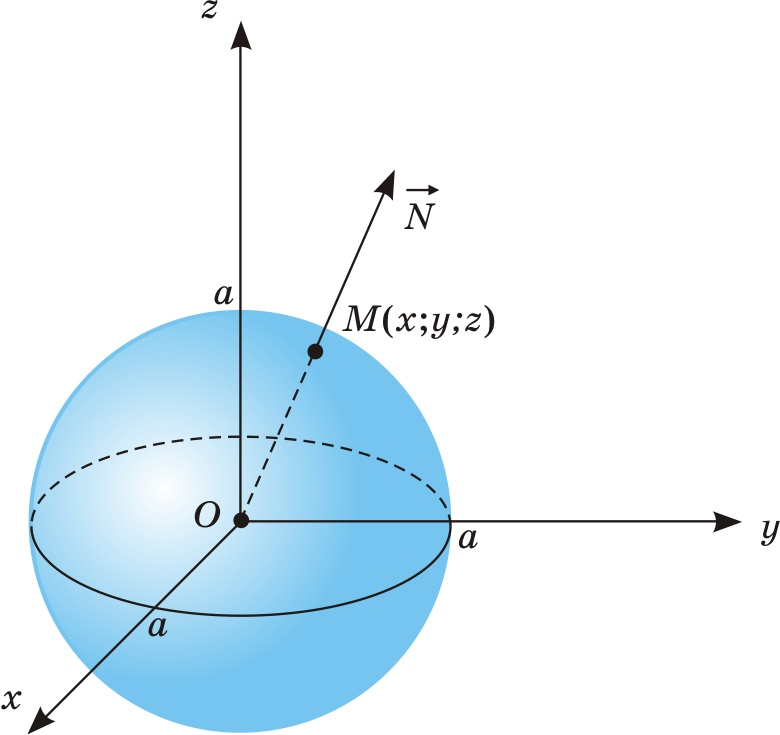
\includegraphics[scale = 0.27]{lec24_1.jpg}
	\end{center}
	
	Этот вектор составляет следующие косинусы с соответствующими осями:
	
	\[\cos\alpha=\frac{x}{a},\quad \cos\beta=\frac{y}{a},\quad \cos\gamma=
	\frac{z}{a}.\]
	
	 Тогда по формуле \eqref{lec24, num_1} переходим к ПовИ-1:
	\[I=\iint\limits_\pi\left(\frac{x^2}{a} + \frac{y^2}{a} +
	 \frac{z^2}{a}\right)ds = a \iint\limits_\pi ds = 4\pi a^3.\]
\end{example}

\section{Связь ПовИ-2 с 3И}

Рассмотрим некоторое тело $V\subset \R^3,$ ограниченное поверхностью $\pi.$ 
Как и ранее, $\pi$~--- гладкая квадрируемая двусторонняя поверхность. 
Под $\pi$ понимают внешнюю сторону этой поверхности. Тогда верна

\begin{thm}[формула Гаусса-Остроградского]
\begin{equation}\label{lec24, num_3}
\boxed{\iint\limits_\pi Pdydz +  Qdxdz + Rdxdy = \iiint\limits_V \left(\pderiv 
{P}{x}
  + \pderiv {Q}{y} + \pderiv{R}{z}\right) dxdydz}\end{equation}
  
   Слева~--- ПовИ-2, справа~--- 3И по области $V$ с границей $\pi$.
\end{thm}

\begin{proof}
Вычислим
\[\iiint\limits_V \pderiv {R(x, y, z)}{z} dxdydz = *\]

Будем предполагать, что $V$ --- такое тело, что любая прямая, параллельная 
$Oz,$
 пересекает поверхность $\pi$ не более, чем в двух точках (строго выпуклое в 
 направлении $Oz$).

\begin{center}
	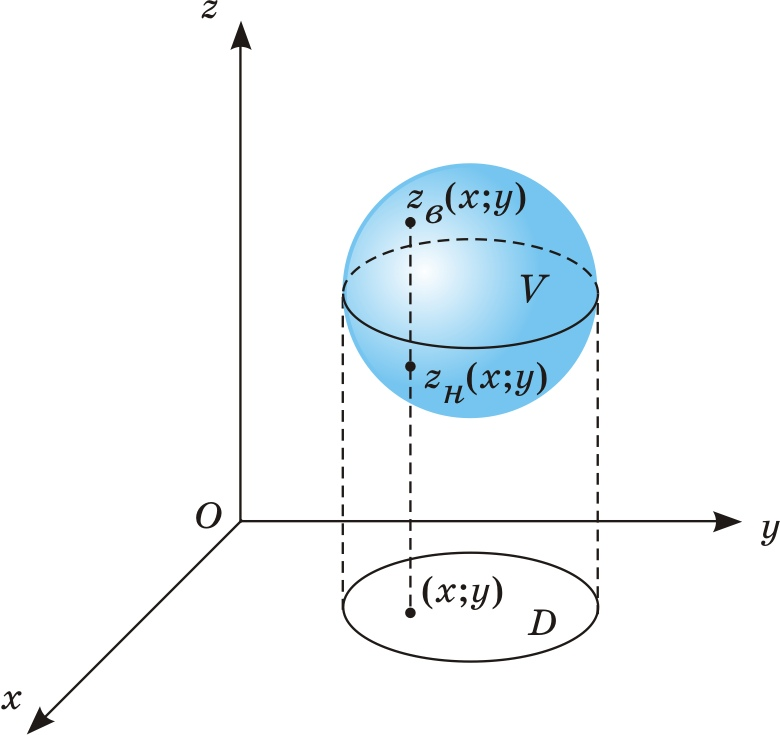
\includegraphics[scale = 0.3]{lec24_2.jpg}
\end{center}

Пусть $D$~--- проекция $V$ на плоскость $Oxy.$ Для каждой точки $(x, y) \in D$ 
построим перпендикуляр. Тогда
  поверхность $\pi$ разобьется на две части: одна будет содержать точки
   $z_{\text{н}},$ вторая~--- точки $z_{\text{в}}.$
Получим части $\pi_{\text{н}}$ и $\pi_{\text{в}}.$
Тогда \begin{multline*}*=\iint\limits_D dxdy\int\limits_{z_{\text{н}}(x,y)}
^{z_{\text{в}}(x, y)}\pderiv{R(x, y, z)}{z}dz = \iint\limits_D dxdy\cdot R(x, 
y, z)
\bigg|_{z=z_{\text{н}}(x, y)}^{z=z_{\text{в}}(x, y)} = \\= \iint\limits_{\pi_
	{\text{в}}^{\uparrow}} R(x, y, z)dxdy - \iint\limits_{\pi_{\text{н}}^
	{\uparrow}} R(x, y, z)dxdy = \iint\limits_{\pi_{\text{в}}^{\uparrow}} 
R(x, y, z)dxdy +  \iint\limits_{\pi_{\text{н}}^{\downarrow}} R(x, y, z)dxdy = 
*\end{multline*}

Второй интеграл --- интеграл по верхней стороне поверхности $\pi_{\text{н}},$
 для которой нормаль направлена внутрь тела $V.$ Поменяв знак перед интегралом 
 c ``$-$'' на ``$+$'',
  мы получили интеграл по внешней стороне поверхности $\pi,$ соответствующий
   $\pi_{\text{н}}.$

\[* = \iint\limits_\pi R(x, y, z)dxdy.\]

Аналогично доказывается, что \[\iiint\limits_V \pderiv {P}{x} dxdydz = \iint
 Pdydz,\quad \iiint\limits_V \pderiv {Q}{y} dxdydz = \iint 
 Qdxdz.\]
В совокупности это дает формулу Гаусса-Остроградского.
\end{proof}

\begin{example}
	Вычислить \[I = \iint\limits_\pi x^3dydz + y^3dxdz + z^3dxdy,\] где $\pi$~---
	внешняя сторона сферы $x^2 + y^2 + z^2 = a^2.$
	 
	Воспользуемся формулой \eqref{lec24, num_3}:
	
	\begin{multline*}I=\iiint\limits_V (3x^2 + 3y^2 + 3z^2)dxdydz = \left[ 
	\begin{cases}x=
	 r\cos\phi \cos\psi,\\ y=r\sin\phi\cos\psi, \\ z=r\sin\psi,\end{cases}
	\begin{gathered}J =r^2\cos\psi,\\ \phi\in[0, 2\pi], \\ 
	\textstyle\psi\in\left[-\frac{\pi}{2},
	  \frac{\pi}{2}\right]\end{gathered}\right]=\\ 
	  =3\int\limits_0^{2\pi}d\phi\int\limits
	  _{-\frac{\pi}{2}}^{\frac{\pi}{2}}\cos\psi d\psi\int\limits_0^a r^4 dr=
	  3\cdot2\pi\cdot2\cdot\frac{a^5}5 = 
	  \frac{12}{5}\pi a^5.\end{multline*}
\end{example}

\end{document}
